
% This LaTeX was auto-generated from MATLAB code.
% To make changes, update the MATLAB code and republish this document.

\documentclass{article}
\usepackage{graphicx}
\usepackage{color}
\usepackage[colorlinks=false, hidelinks=true]{hyperref}

\sloppy
\definecolor{lightgray}{gray}{0.5}
\setlength{\parindent}{0pt}

\begin{document}

    
    
\subsection*{Contents}

\begin{itemize}
\setlength{\itemsep}{-1ex}
   \item Setup
   \item Part a
   \item Part b
   \item Part c: Inverse Filtering in Frequency domain
   \item Part d
   \item Find threshold for noisy reconstruction
\end{itemize}


\subsection*{Setup}

\begin{verbatim}
close all;
clc;
\end{verbatim}


\subsection*{Part a}

\begin{verbatim}
I = imread('cameraman.tif');
X = im2double(I);
X = X(50:80,105:138);
F = gauss2d(9,9,0,0,2,2);
figure
surf(F)
title('Gaussian Filter')
C = convmtx2(F,size(X,1),size(X,2));
X_vec = X(:);
y = C*X_vec;
f1 = figure;
ax = gca;
subplot(2,2,1,ax)
imagesc(X), colormap gray
title('Original Phantom')
subplot(2,2,2)
Y_blurred = reshape(y,size(F)+size(X)-1);
imagesc(Y_blurred)
title('Blurred Phantom')
\end{verbatim}

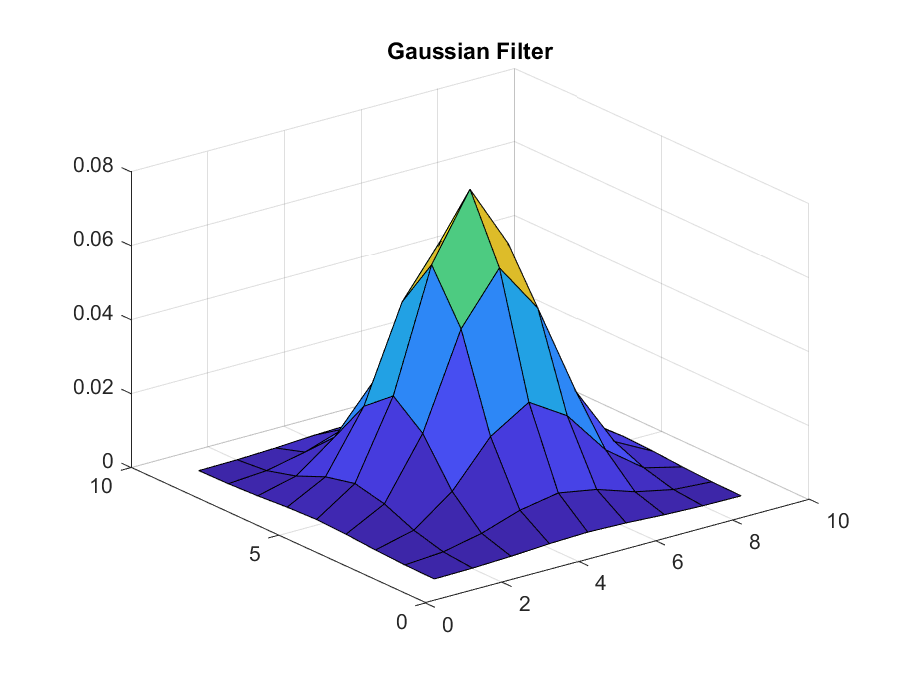
\includegraphics [width=4in]{Q3_01.eps}

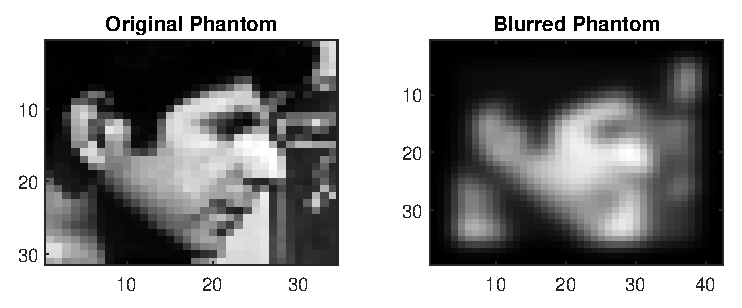
\includegraphics [width=4in]{Q3_02.eps}


\subsection*{Part b}

\begin{verbatim}
for ratio = [3 4]
    variance = var(y)/10^ratio; % SNR adjustment
    sigma_n = sqrt(variance);
    noise = sigma_n * randn(size(y)); % N~(0,sigma_n^2)
    y_n = y + noise;
    y_img = reshape(y_n,size(F)+size(X)-1);
    subplot(2,2,ratio)
    imagesc(y_img)
    title(['Blurred Phantom with SNR: ',num2str(10*ratio)])
end
\end{verbatim}

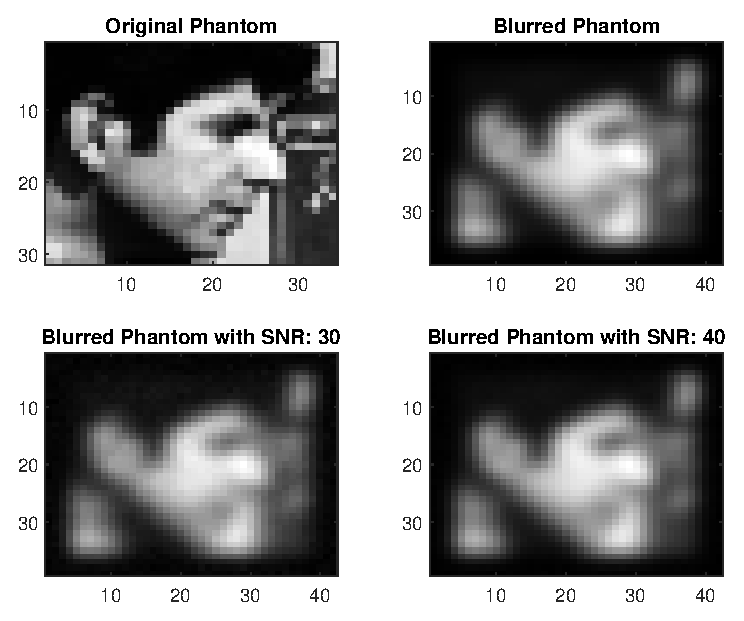
\includegraphics [width=4in]{Q3_03.eps}

\subsubsection*{Comments}
The effect of the noise is not observable to human eye under the effect of blurring, \textit{i.e.} it is difficult to distinguish the noise from the blurred image. 


\subsection*{Part c: Inverse and LS Filtering in Frequency domain}

\begin{verbatim}
figure
size_Y = size(Y_blurred);
X_inv = ifft2(fft2(Y_blurred,size_Y(1), ...
    size_Y(2))./fft2(F,size_Y(1),size_Y(2)),size_Y(1),size_Y(2));
X_inv_noisy = ifft2(fft2(y_img)./fft2(F, ...
    size_Y(1),size_Y(2)),size_Y(1),size_Y(2));
subplot(1,2,1)
imagesc(X_inv), colormap gray
title('Inverse Filtering of y')
subplot(1,2,2)
imagesc(X_inv_noisy)
title('Inverse Filtering of y_{noise}')

figure
C = full(C); % The LS solution outputs wrong results if C remains sparse!
X_inv = reshape(inv(C'*C)*C'*y,size(X));
X_inv_noisy = reshape(inv(C'*C)*C'*y_n,size(X));
subplot(1,2,1)
imagesc(X_inv), colormap gray
title('Least Squares Filtering of y')
subplot(1,2,2)
imagesc(X_inv_noisy)
title('Least Squares Filtering of y_{noise}')
\end{verbatim}

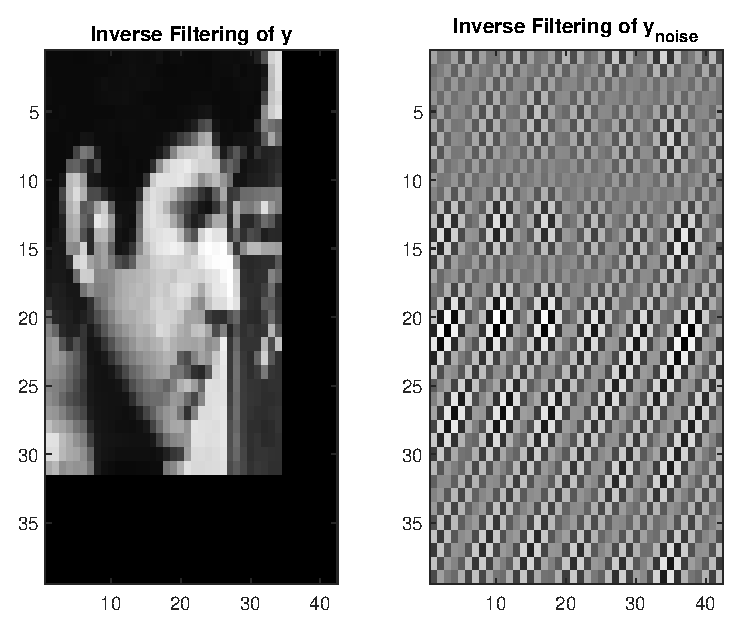
\includegraphics [width=4in]{Q3_04.eps}

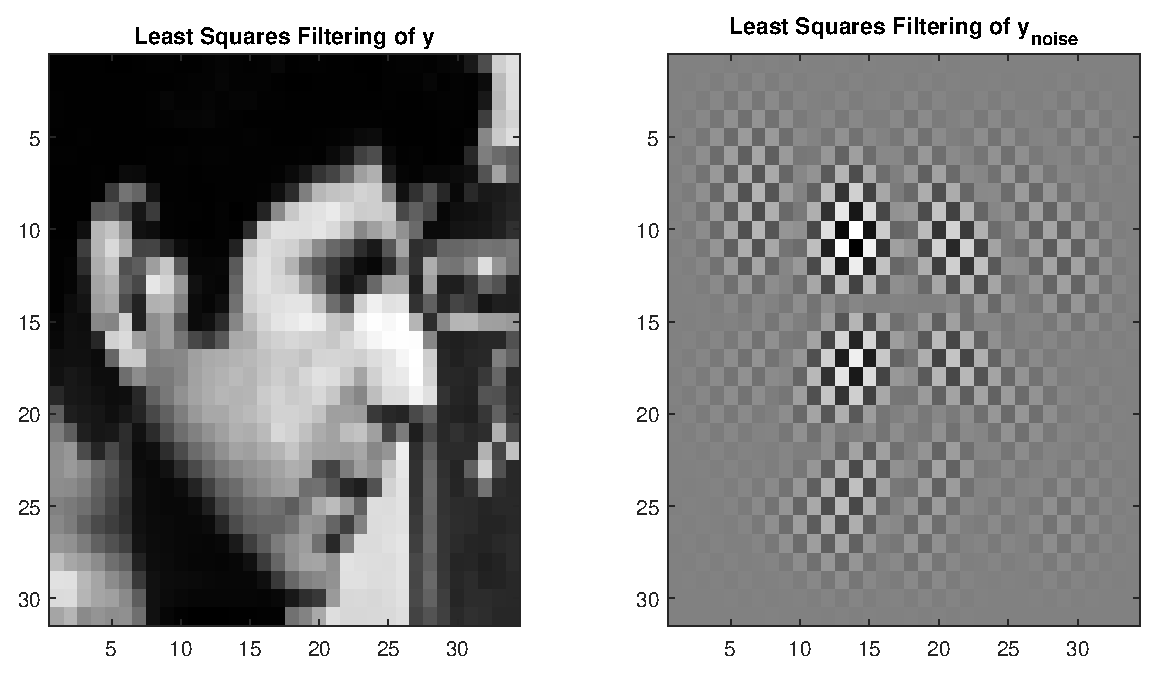
\includegraphics [width=4in]{Q3_05.eps}

\subsubsection*{Comments}

\begin{eqnarray}
    \tilde{y} &= y + n \\
    A &= U{\Sigma}V^H \label{eqn:SVD1}\\
    A^T &= V{\Sigma}U^H \label{eqn:SVD2}\\
    \hat{x_{LS}} &= (A^TA)^{-1}A^T \label{eqn:LS}
\end{eqnarray}
Inserting Eqn. \ref{eqn:SVD1} and \ref{eqn:SVD2} in \ref{eqn:LS}, results in following expression:
\begin{equation}
    \hat{x_{LS}} = \underbrace{V{\Sigma}^{-1}U^H}_{A^{\dagger}}(y+n)
\end{equation}
The least squares solution amplifies the noise with pseudo-inverse of A (in SVD sense) hence results in the checkerboard pattern in the reconstruction as an implication of amplified high frequency noise. Since A is an ill-conditioned matrix and hence has really small singular values, noise is amplified with $\frac{1}{\sigma}$ which is a huge amplification factor. 

\subsection*{Part d}

\begin{par}
y = U S VH x; x = V 1/S UH y;
\end{par} \vspace{1em}
\begin{verbatim}
[U,S,V] = svd(C);
singular_values = diag(S);
X_back_vec = zeros(size(X_vec));
Errors = zeros(size(singular_values));
for i = 1:length(singular_values)
    s = singular_values(i);
    v = V(:,i);
    u = U(:,i);
    X_back_vec = X_back_vec + 1/s * v * u' * y;
    Errors(i) = relative_error(X_vec, X_back_vec);
end
X_back = reshape(X_back_vec,size(X));
f = figure;
f.Position = [100 100 900 300];
colormap gray
subplot(1,3,1)
imagesc(X)
title('Original Image')
subplot(1,3,2)
imagesc(X_back)
title('Reconstructed Image')
subplot(1,3,3)
plot(Errors)
title('Errors')
sgtitle('TSVD Reconstructions for noiseless image')

[U,S,V] = svd(C);
singular_values = diag(S);
X_back_vec = zeros(size(X_vec));
Errors = zeros(size(singular_values));
for i = 1:length(singular_values)
    s = singular_values(i);
    v = V(:,i);
    u = U(:,i);
    X_back_vec = X_back_vec + 1/s * v * u' * y_n;
    Errors(i) = relative_error(X_vec, X_back_vec);
end
Full_Errors = Errors;
X_back = reshape(X_back_vec,size(X));
f = figure;
f.Position = [100 100 900 300];
colormap gray
subplot(1,3,1)
imagesc(X)
title('Original Image')
subplot(1,3,2)
imagesc(X_back)
title('Reconstructed Image')
subplot(1,3,3)
plot(Errors)
title('Errors')
sgtitle('TSVD Reconstructions for noisy image')
\end{verbatim}

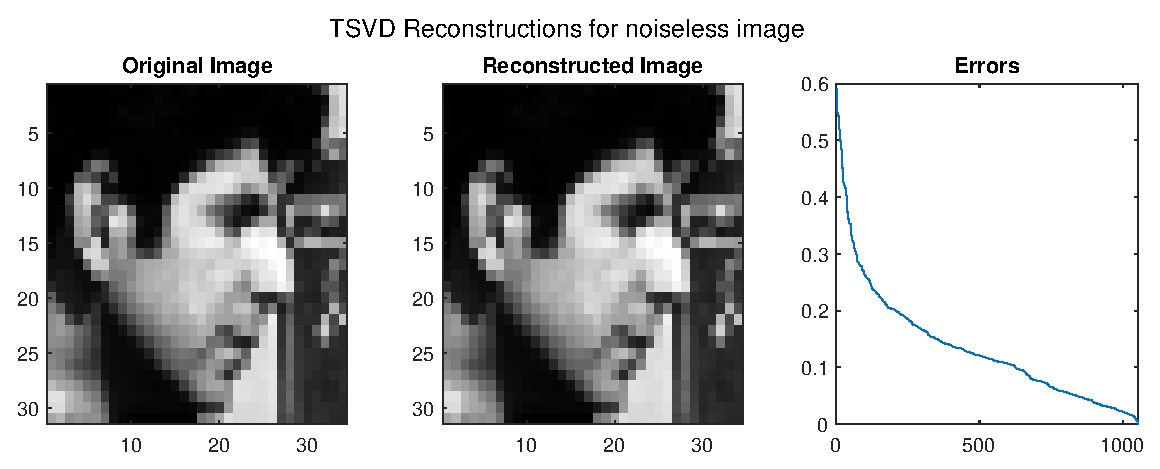
\includegraphics[width=4in]{Q3_06.eps}

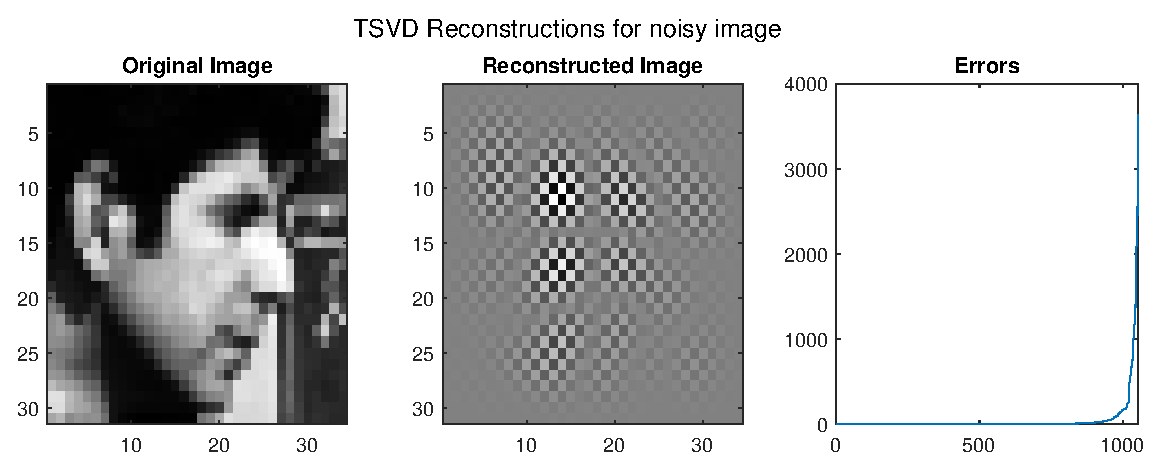
\includegraphics [width=4in]{Q3_07.eps}\label{fig:noise_tsvd}

\subsubsection*{Comments}

For this question a distance error metric is defined: 

\begin{equation}
    Relative Error = \frac{||\hat{x}-x||}{||x||}
\end{equation}
In the figure above, we observe that error is growing after the 900th singular value. Hence, to find a suitable threshold, this interval is scanned.

\subsection*{Find threshold for noisy reconstruction}

\begin{par}
A ratio of $\frac{1}{200}$ in singular value amplitude provided a satisfactory amount of reconstruction.
\end{par} \vspace{1em}
\begin{verbatim}
f = figure; colormap gray;
f.Position = [100 100 600 800];
plot_idx = 4;
for ratio = 100:100:900
    max_sing_value = max(singular_values);
    threshold = max_sing_value / ratio;
    [minimum, index] = min(abs(singular_values-threshold));

    X_back_vec = zeros(size(X_vec));
    Errors = zeros(index,1);
    for i = 1:index
        s = singular_values(i);
        v = V(:,i);
        u = U(:,i);
        X_back_vec = X_back_vec + 1/s * v * u' * y_n;
        Errors(i) = relative_error(X_vec, X_back_vec);
    end
    X_back = reshape(X_back_vec,size(X));
    subplot(4,3,plot_idx)
    imagesc(X_back)
    title({['Ratio:',num2str(ratio)] ...
        ,['Min Eigenvalue index: ',num2str(index)]})
    plot_idx = plot_idx + 1;
end

colormap gray
subplot(4,3,1)
imagesc(X)
title('Original Image')

subplot(4,3,2)
plot(100:900,Full_Errors(100:900))
title('Errors')
xlabel('Singular Value Iteration')
ylabel('Relative Error')

subplot(4,3,3)
plot(singular_values)
title('Sorted Singular Value distribution')
sgtitle('TSVD Reconstructions for noisy image')
\end{verbatim}

\includegraphics [width=4in]{Q3_08.eps}

\subsubsection*{Comments}
Experiments showed that applying a threshold around the 1\% of the maximum singular value resulted in moderate success when compared to the other reconstruction thresholds. The corresponding singular value index is found to be 433. This can also be seen in the error plot given in the top of the above figure, where error gets drastically higher after the inclusion of 500 singular values. 

\pagebreak

\section*{Conjugate Gradient}

\subsubsection*{Comments}

As stated, the main intensive task in the Conjugate gradient method is the repetitive forward operators. Tikhonov regularized solution can be found by assigning $A=(C^TC+{\lambda}D^TD)$. However, this may not be useful in memory-limited systems. Hence forward projections of A should be replaced with another operation requiring less memory. This can be done as follows:
\begin{eqnarray}
    Az &= (C^TC+{\lambda}D^TD)z \\ 
    &= C^T(Cz)+ {\lambda}D^T(Dz) \label{eqn:fastforward}
\end{eqnarray}

The quantities $Cz$ and $C^Tz$ in Eqn.~\ref{eqn:fastforward} can be computed using fast-forward routines, keeping in mind that the operator $C$ represents convolution operation, hence it can be computed via FFTs. Hence, one only needs to store the discrete derivative operator and reduces memory requirements drastically. 
\end{document}

